%\documentclass[tikz,convert={outfile=\jobname.svg},border=5pt]{standalone}
\documentclass[tikz,border=15pt]{standalone}
\usepackage[utf8x]{inputenc}
\usetikzlibrary{positioning}
\usetikzlibrary{decorations.text}
% To create the .png:
% > pdflatex fig1.tex
% > convert -density 300 fig1.pdf -quality 100 fig1.png

\begin{document}
    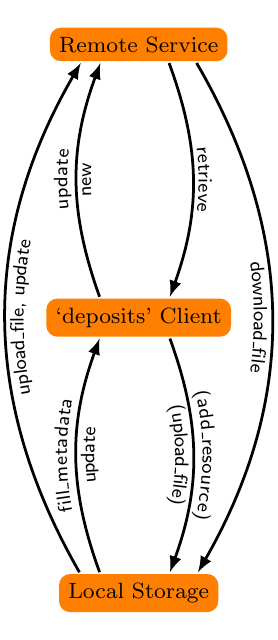
\begin{tikzpicture}[font=\footnotesize]
        \tikzstyle{node_style} = [rounded corners, rectangle, fill=orange]
        \tikzstyle{arrow_style1} = [->, black, line width=1, >=latex, shorten <=0.5pt, shorten >=0.5pt]

        \node[node_style] (n1) {Local Storage};
        \node[node_style] (n2) [above=3cm of n1] {`deposits' Client};
        \node[node_style] (n3) [above=3cm of n2] {Remote Service};

        \draw [
            arrow_style1,
            postaction={
                decorate,
                decoration={
                    raise=0.8ex,
                    text along path,
                    text align=center,
                    text={|\sffamily\scriptsize|fill{\_}metadata}
                }
            },
            postaction={
                decorate,
                decoration={
                    raise=-1.5ex,
                    text along path,
                    text align=center,
                    text={|\sffamily\scriptsize|update}
                }
            },
            transform canvas={xshift=-4mm}
        ] (n1) to [bend left=20]  (n2);

        \draw [
            arrow_style1,
            postaction={
                decorate,
                decoration={
                    raise=0.8ex,
                    text along path,
                    text align=center,
                    text={|\sffamily\scriptsize|(add{\_}resource)}
                }
            },
            postaction={
                decorate,
                decoration={
                    raise=-1.5ex,
                    text along path,
                    text align=center,
                    text={|\sffamily\scriptsize|(upload{\_}file)}
                }
            },
            transform canvas={xshift=3mm}
        ] (n2) to [bend left=20]  (n1);

        \draw [
            arrow_style1,
            postaction={
                decorate,
                decoration={
                    raise=0.8ex,
                    text along path,
                    text align=center,
                    text={|\sffamily\scriptsize|update}
                }
            },
            postaction={
                decorate,
                decoration={
                    raise=-1.2ex,
                    text along path,
                    text align=center,
                    text={|\sffamily\scriptsize|new}
                }
            },
            transform canvas={xshift=-4mm}
        ] (n2) to [bend left=20]  (n3);

        \draw [
            arrow_style1,
            postaction={
                decorate,
                decoration={
                    raise=0.5ex,
                    text along path,
                    text align=center,
                    text={|\sffamily\scriptsize|retrieve}
                }
            },
            transform canvas={xshift=3mm}
        ] (n3) to [bend left=20]  (n2);


        \draw [
            arrow_style1,
            postaction={
                decorate,
                decoration={
                    raise=-1.5ex,
                    text along path,
                    text align=center,
                    text={|\sffamily\scriptsize|upload{\_}file, update}
                }
            },
            transform canvas={xshift=-6mm}
        ] (n1) to [bend left=30]  (n3);

        \draw [
            arrow_style1,
            postaction={
                decorate,
                decoration={
                    raise=-1.5ex,
                    text along path,
                    text align=center,
                    text={|\sffamily\scriptsize|download{\_}file}
                }
            },
            transform canvas={xshift=6mm}
        ] (n3) to [bend left=30]  (n1);

    \end{tikzpicture}

\end{document}
